%% This is file `DEMO-TUDaReport.tex' version 4.00 (2025-01-26),
%% it is part of
%% TUDa-CI -- Corporate Design for TU Darmstadt
%% %%%%%%%%%%%%%%%%%%%%%%%%%%%%%%%%%%%%%%%%%%%%%%%%%%%%%%%%%%%%%%%%%%%%%%---------------
%%
%% Copyright (C) 2018--2025 by Marei Peischl <marei@peitex.de>
%%
%% ============================================================================
%% This work may be distributed and/or modified under the
%% conditions of the LaTeX Project Public License, either version 1.3c
%% of this license or (at your option) any later version.
%% The latest version of this license is in
%% http://www.latex-project.org/lppl.txt
%% and version 1.3c or later is part of all distributions of LaTeX
%% version 2008/05/04 or later.
%%
%% This work has the LPPL maintenance status `maintained'.
%%
%% The current maintainer of this work is
%%   Marei Peischl <tuda-ci@peitex.de>
%%
%% The development repository can be found at
%% https://github.com/tudace/tuda_latex_templates
%% Please use the issue tracker for feedback!
%%
%% If you need a compiled version of this document, have a look at
%% http://mirror.ctan.org/macros/latex/contrib/tuda-ci/doc
%% or at the documentation directory of this package (if installed)
%% <path to your LaTeX distribution>/doc/latex/tuda-ci
%% ============================================================================
%%
% !TeX program = lualatex
%%

\documentclass[
	german,% Main language as global option
	accentcolor=3d,% Choose accent color: For a list of available colors see the full tudapub documentation
	type=intern, % Minimal setup without accent color
	marginpar=false,% Disable marginpar
%	accept-missing-logoes=true,% No error in case logo files are not available
%	logofile=example-image,% In case logo should be replaced
]{tudapub}


%%%%%%%%%%%%%%%%%%%
% Language setup
%%%%%%%%%%%%%%%%%%%
\usepackage[german]{babel}
\usepackage[autostyle]{csquotes}% \enquote, to simplify use of quotation marks
\usepackage{amsmath}
\usepackage{graphicx}
\usepackage{wrapfig}
\usepackage[justification=centering]{caption}
\usepackage{tikz}
\usetikzlibrary{arrows.meta, positioning, calc, quotes, decorations.pathmorphing}
\usepackage{pgfplots}
\usepackage{musicography}
\usepackage{xcolor}

\tikzset{>=Latex}

\title{Versuch Doppler-Sonographie}
\subtitle{Theorie}
%\date{}% If not specified, today's date is automatically inserted


\begin{document}

\maketitle
\tableofcontents
% Additional lists like \listoffigures or acronyms might be added here
\newpage

\section{Hämodynamische Grundlagen}\label{sec:haemodynamische-grundlagen}

   Ultraschall-Doppler-Verfahren werden in der Medizin unter anderem eingesetzt, um Flussgeschwindigkeiten in Gefäßen zu erfassen. Aus den Ergebnissen solcher Untersuchungen lassen sich Aussagen über Organdurchblutung und Gefäßmorphologie ableiten. Um die Geschwindigkeitsinformationen in Bezug auf diese Anwendungsgebiete interpretieren zu können, werden sogenannte hämodynamische Modelle verwendet. Sie modellieren die physikalischen Zusammenhänge des Blutflusses in Gefäßen von Lebewesen. Im Folgenden wird ein stark vereinfachtes Modell des Herz-Kreislauf-Systems vorgestellt, das ausreicht, um Dopplerbefunde als mögliche pathologische Phänomene zu interpretieren.

   \begin{figure}[htbp]
      \centering
      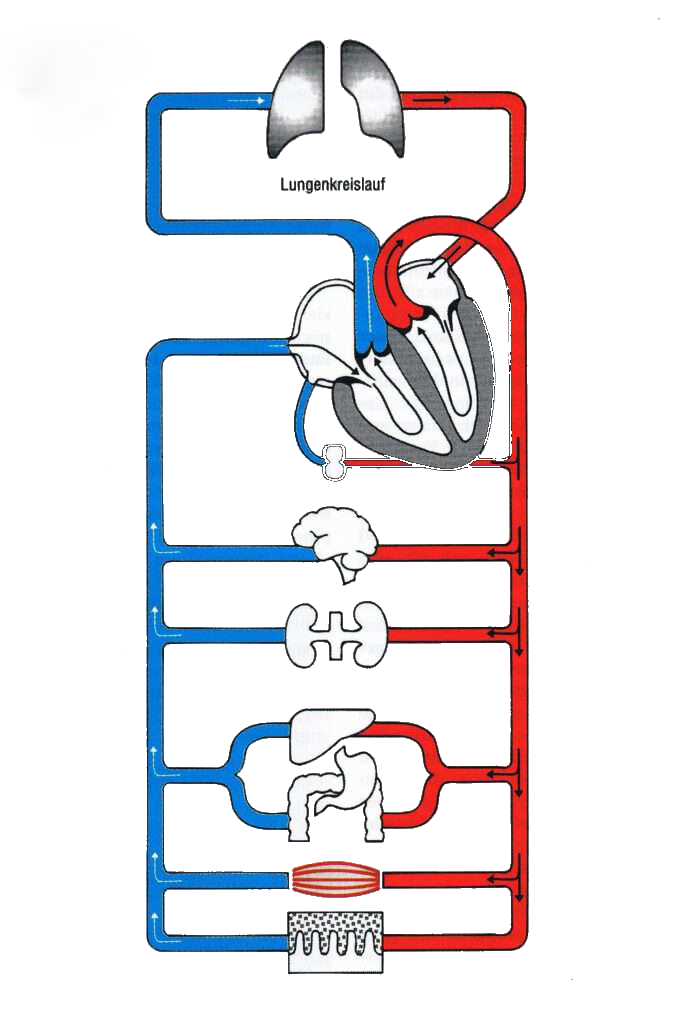
\includegraphics[width=0.4\textwidth]{hks.png}
      \caption{Vereinfachtes hämodynamisches Modell des Herz-Kreislauf-Systems.}\label{fig:herz-kreislauf-modell}
      % Quelle hks https://schwimmlexikon.de/herz-kreislaufsystem/
   \end{figure}

\subsection{Herz-Kreislauf-System}\label{sec:herz-kreislauf}

   Das Herz-Kreislauf-System kann vereinfacht als geschlossenes Röhrensystem aufgefasst werden, wie in Abbildung~\ref{fig:herz-kreislauf-modell} schematisch dargestellt. Es besteht aus zwei Kreisläufen: dem kleineren Lungenkreislauf und dem größeren Körperkreislauf. Beide Kreisläufe sind in Reihe geschaltet, der gemeinsame Verknüpfungspunkt ist das Herz. Im Körperkreislauf sind die einzelnen Organe (z.B.\ Gehirn, Nieren oder Skelettmuskulatur) über Gefäßwiderstände parallel zueinander geschaltet. 
   \\
   In dieser Analogie übernimmt das Herz die Rolle der antreibenden Druckquelle. Es sorgt dafür, dass das Blut als Transportmedium für Sauerstoff, Nährstoffe und Stoffwechselprodukte durch den Körper gepumpt wird. Aufgrund der rhythmischen Herzaktion ist die Strömung im Gefäßsystem nicht kontinuierlich, sondern pulsatil. Während der Systole wird Blut aus dem Herzen in die Arterien ausgeworfen, während der Diastole füllt sich das Herz wieder. Form und Höhe des Druck- und Flussverlaufs werden durch die Eigenschaften von Herz und Gefäßen gemeinsam bestimmt.
   \\
   Zwischen Blutvolumenstrom \(Q\), Gefäßwiderstand \(R\) und Druckdifferenz \(P\) besteht eine Beziehung, die formal der Analogie zum ohmschen Gesetz im elektrischen Schaltkreis entspricht:
   \[
      Q = \frac{P}{R} \, .
   \]
   Zum Vergleich gilt im elektrischen Schaltkreis
   \[
      I = \frac{U}{R} \, .
   \]

   Der Volumenstrom \(Q\) beschreibt, welches Volumen eines Mediums (hier Blut) pro Zeitspanne durch eine bestimmte Querschnittsfläche \(A\) transportiert wird. Bei gegebener mittlerer Strömungsgeschwindigkeit \(\bar{v}_A\) und Querschnittsfläche \(A\) gilt
   
   \begin{equation}
      Q = \bar{v}_A \cdot A \, .
      \label{eq:volumenstrom}
   \end{equation}

   In Tabelle~\ref{tab:flussgeschwindigkeiten} sind typische Querschnittsflächen sowie maximale und mittlere Flussgeschwindigkeiten für verschiedene Gefäßtypen des menschlichen Körpers aufgeführt.

   \begin{table}[htbp]
      \centering
      \renewcommand{\arraystretch}{1.3}
      \begin{tabular}{lccc}
         Gefäßtyp & $A\,[\mathrm{cm}^2]$ & $v_{\max}\,[\mathrm{cm/s}]$ & $\bar{v}_A\,[\mathrm{cm/s}]$ \\ \hline
         Arterie & bis zu $1,56$ & bis zu $100$ & bis zu $25$ \\
         Arteriole & $4 \mu  \;-\; 25 \mu$ & $1 \;-\; 2$ & bis zu $1$ \\
         Terminale Arteriole & $1 \mu \;-\; 4 \mu$ & $0{,}2 \;-\; 0{,}3$ & bis zu $0{,}2$ \\
         Kapillare & $0{,}0225 \mu \;-\; 0{,}16 \mu$ & $0{,}02 \;-\; 0{,}05$ & bis zu $0{,}05$ \\ \hline
      \end{tabular}
      \caption{Übersicht über maximale und mittlere Flussgeschwindigkeiten in verschiedenen Gefäßen.}\label{tab:flussgeschwindigkeiten}
   \end{table}

   Der Gefäßwiderstand eines Gefäßsegments lässt sich bei laminaren, stationären Strömungen eines newtonschen Fluids mit Hilfe des Hagen--Poiseuille-Gesetzes beschreiben:
   \begin{equation}
      \frac{1}{R} = \frac{\pi r^{4}}{8 \,\eta\, l} \, .
      \label{eq:hagen-poiseuille}
   \end{equation}
   
   Hierbei ist \(r\) der Gefäßradius, \(\eta\) die Viskosität des Blutes und \(l\) die Länge des betrachteten Gefäßabschnitts. Der Zusammenhang zeigt, dass bereits kleine Änderungen des Gefäßradius einen starken Einfluss auf den Widerstand haben, da der Radius mit der vierten Potenz einhergeht.
   \\
   Im pathologischen Fall einer Gefäßverengung (Stenose) kommt es zunächst zu einer Zunahme der Strömungsgeschwindigkeit im verengten Bereich. Ab einem bestimmten Stenosegrad steigt jedoch der Widerstand so stark an, dass trotz unverändertem oder sogar erhöhtem Blutdruck der Blutfluss hinter der Stenose abnimmt. Diese Veränderungen des Strömungsverhaltens sind für die Interpretation hämodynamischer Messgrößen, etwa aus Doppler-Ultraschallbefunden, von zentraler Bedeutung.

\subsection{Strömungsprofile}\label{sec:stroemungsprofile}

   Im Allgemeinen wird innerhalb von Gefäßen des menschlichen Körpers zwischen zwei grundlegenden Strömungsformen unterschieden: laminarer und turbulenter Strömung (siehe Abbildung~\ref{fig:laminar-turbulent}).

   \begin{figure}[htbp]
      \centering
      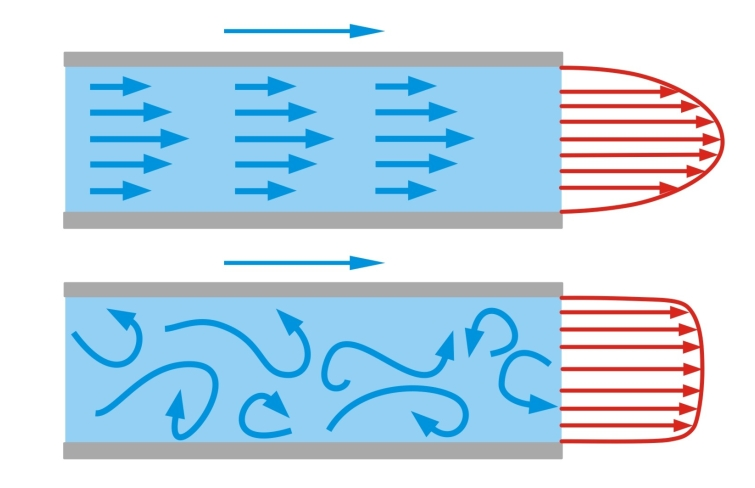
\includegraphics[width=0.6\textwidth]{stroemungsprofile.jpg}
      \caption{Laminare und turbulente Strömungsprofile in einem Gefäßquerschnitt.}\label{fig:laminar-turbulent}
      % Quelle stroemngsprofile https://www.gunt.de/de/produkte/rohrreibung-bei-laminarer-turbulenter-stroemung/070.15001/hm150-01/glct-1:pa-119:pr-548
   \end{figure}

   Bei laminarer Strömung nimmt die Geschwindigkeit der Blutschichten von der Gefäßwand zur Gefäßachse hin zu. Die Flüssigkeitsteilchen, die sich direkt an der Gefäßwand befinden, sind praktisch in Ruhe, während die Teilchen im Axialstrom die höchste Geschwindigkeit aufweisen. Es bildet sich ein parabolisches Strömungsprofil aus (siehe Abbildung~\ref{fig:laminar-turbulent}). 
   \\
   Bei turbulenter Strömung verläuft die Strömungsrichtung hingegen nicht mehr geordnet parallel zur Achse. Statt eines parabolischen ergibt sich ein abgeflachtes, unregelmäßiges Strömungsprofil. Dieser veränderte Strömungsverlauf ist mit einem erhöhten Strömungswiderstand verbunden und kann im pathologischen Fall zu einer zusätzlichen Druckbelastung des Herzens beitragen.
   \\
   Ob sich in einem Gefäß eine laminare oder turbulente Strömung einstellt, hängt von verschiedenen Faktoren ab. Eine Rolle spielen insbesondere Flussgeschwindigkeit, Gefäßradius, Dichte und Viskosität der Flüssigkeit. Mit Hilfe der sogenannten Reynoldsschen Zahl lässt sich für konkrete Situationen abschätzen, ob in einem Gefäß eher eine laminare oder eine turbulente Strömung zu erwarten ist.
   \\
   Turbulente Strömungen erzeugen Strömungsgeräusche, während laminare Strömungen nahezu geräuschlos sind. Diese Geräusche sind für die Auskultation von großer Bedeutung: Die normalen Herztöne entstehen in erster Linie durch die Vibrationen, die der plötzliche Verschluss der Herzklappen sowie die daraus resultierenden Beschleunigungen des Blutes und der Herzwand verursacht. Dieser Vorgang geht mit transienten Turbulenzen einher. Pathologische Strömungsgeräusche, wie sie z.B. bei Klappenfehlern oder Querschnittsveränderungen bei Gefäßstenosen auftreten, werden direkt durch anhaltende turbulente Strömungen ausgelöst; die dabei entstehenden Geräusche lassen sich mit dem Stethoskop auskultieren.

\section{Physikalische Grundlagen des Ultraschall-Dopplers}\label{sec:physik-doppler}

   In diesem Abschnitt werden die physikalischen Grundlagen des Ultraschall-Dopplers erläutert. Dazu wird zunächst beschrieben, wie Schall und insbesondere Ultraschall erzeugt wird. Anschließend wird der Doppler-Effekt als Ursache der frequenzbasierten Geschwindigkeitsmessung dargestellt.

   \subsection{Schallerzeugung und -ausbreitung}\label{sec:schallerzeugung-und-ausbreitung}

      Als Schall werden mechanische Schwingungen in einem elastischen Medium bezeichnet. Im Allgemeinen werden sie von einem schwingenden Körper erzeugt und breiten sich von dort in Form von Schallwellen aus. Die Bewegung des schwingenden Körpers überträgt sich auf das umgebende Medium (z.B.\ Luft), das dabei abwechselnd komprimiert und gedehnt wird (vgl. Abbildung~\ref{fig:schallwelle}). Es entstehen Zonen mit Über- und Unterdruck, die sich im Medium fortpflanzen.

      \begin{figure}[htbp]
         \centering
         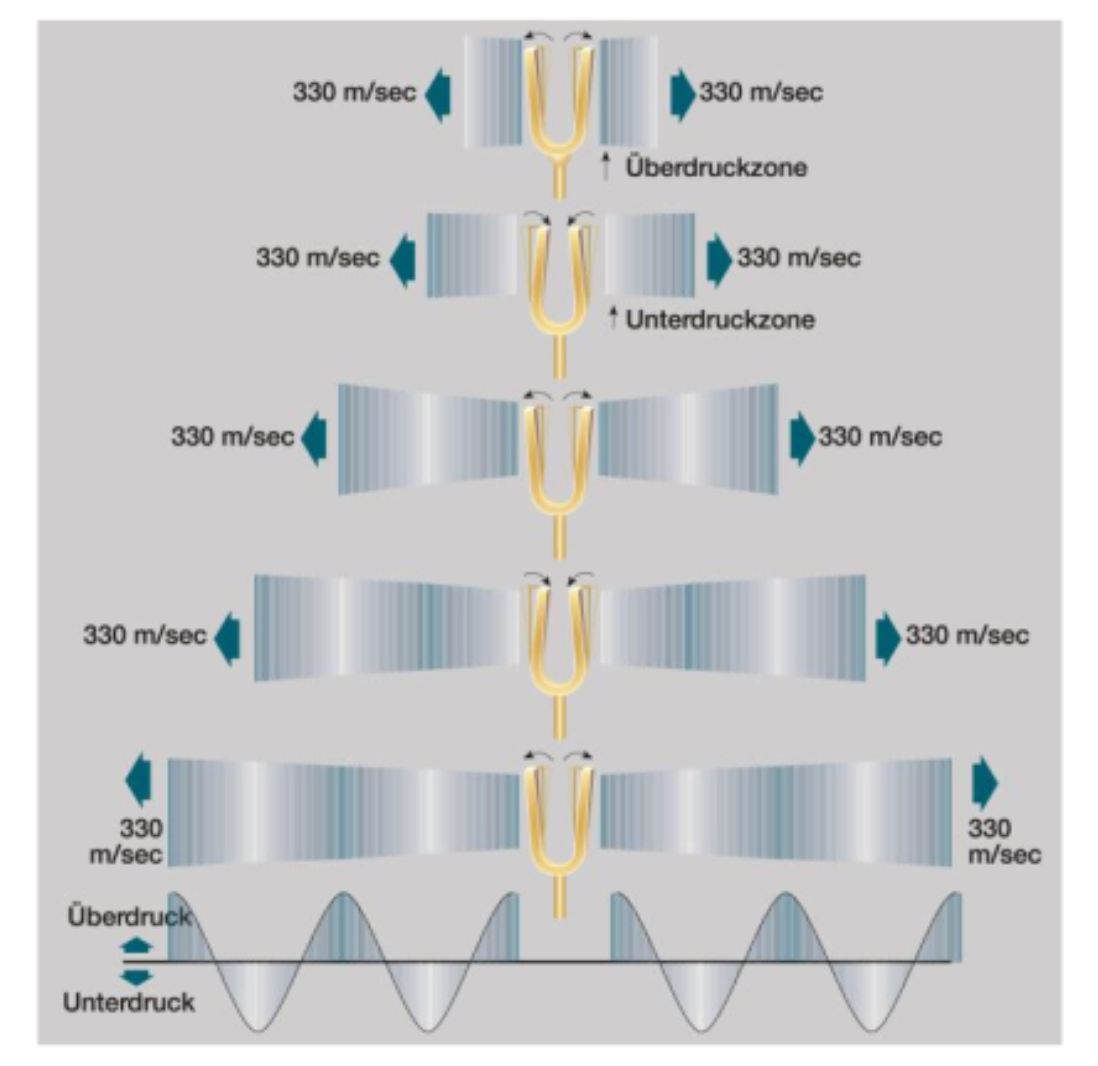
\includegraphics[width=0.6\textwidth]{schall.png}
         \caption{Schematische Darstellung einer Schallwelle.}\label{fig:schallwelle}
      \end{figure}

      Die Ausbreitungsgeschwindigkeit \(c\) des Schalls hängt wesentlich vom jeweiligen Medium ab. In Tabelle~\ref{tab:schallgeschwindigkeiten} sind beispielhaft typische Schallgeschwindigkeiten in verschiedenen Medien zusammengestellt.

      \begin{table}[htbp]
         \centering
         \renewcommand{\arraystretch}{1.3}
         \begin{tabular}{lc}
            Medium & Geschwindigkeit \(c\) [m/s] \\ \hline
            Luft & 330 \\
            Wasser & 1480 \\
            Weichteilgewebe & ca.\ 1540 \\
            Knochen & 2700--4100 \\ \hline
         \end{tabular}
         \caption{Schallgeschwindigkeiten in unterschiedlichen Medien.}\label{tab:schallgeschwindigkeiten}
      \end{table}

      Die Frequenz \(f\) einer Welle beschreibt die Anzahl der vollständigen Schwingungen pro Zeiteinheit und wird üblicherweise in der Einheit Hertz (Hz = 1/s) angegeben. Schwingt beispielsweise eine Violine \(4000\)-mal pro Sekunde, so entsteht ein Ton mit der Frequenz \(f = 4\,\mathrm{kHz}\). Eine rein harmonische (sinusförmige) Schwingung kann als Funktion der Zeit \(t\) näherungsweise durch
      \[
         u(t) = \hat{u}\,\sin(2\pi f t)
      \]
      beschrieben werden, wobei \(\hat{u}\) die Amplitude der Schwingung ist.
      \\
      Mit
      \begin{equation}
         T = \frac{1}{f}
         \label{eq:periode}
      \end{equation}
      wird die Schwingungsdauer \(T\) bezeichnet. Sie gibt die zeitliche Dauer einer kompletten Schwingung einer Welle mit der Frequenz \(f\) an.
      \\
      Die Wellenlänge \(\lambda\) ist die kleinste Distanz zwischen zwei Punkten gleicher Phase 
      (z.B.\ zwischen zwei aufeinanderfolgenden Maxima) einer Welle. Bei gegebener Ausbreitungsgeschwindigkeit \(c\) des Schalls in einem Medium und der Frequenz \(f\) der Schwingung ergibt sich die Wellenlänge zu
      \begin{equation}
         \lambda = \frac{c}{f} \, .
         \label{eq:wellenlaenge}
      \end{equation}
      Damit ist bei bekannter Schallgeschwindigkeit und Frequenz die Wellenlänge eindeutig bestimmt.


   \subsection{Ultraschall}\label{sec:ultraschall}

      Das Gehör des Menschen kann Schallereignisse in einem Frequenzbereich von etwa 16 Hz bis 20 kHz wahrnehmen. Frequenzen unterhalb dieses Bereichs werden als Infraschall, Frequenzen oberhalb als Ultraschall bezeichnet. Ultraschall mit hohen Frequenzen im Bereich von ungefähr 1 bis 20 MHz wird in der medizinischen Diagnostik eingesetzt, unter anderem in der Doppler-Sonographie. Zur Erzeugung von Schall mit derart hohen Frequenzen werden piezoelektrischeKristalle verwendet, häufig in Form dünner Quarz- oder Keramikscheiben. Wird an eine solche Scheibe eine elektrische Spannung angelegt, verformt sich der Kristall: er wird abhängig von Betrag und Polarität der Spannung dicker oder dünner. Bei umgekehrter Polarität erfolgt die Verformung in die entgegengesetzte Richtung. Legt man eine Wechselspannung an, ändert sich die Polarität periodisch; der Kristall beginnt im Rhythmus der Wechselspannung zu schwingen und erzeugt so Ultraschallwellen mit einer definierten Frequenz.
      \\
      Umgekehrt lassen sich piezoelektrische Kristalle auch zum Empfangen von Ultraschall verwenden. Treffen Ultraschallwellen auf den Kristall, führen die Wechselanteile des Schalldrucks zu einer periodischen mechanischen Verformung. Diese Verformung bewirkt eine Ladungsverschiebung im Material und erzeugt eine messbare Wechselspannung an den Elektroden des Kristalls. Dieses Zusammenspiel von mechanischer Verformung und elektrischer Spannung wird als piezoelektrischer Effekt bezeichnet und wurde 1880 von den Geschwistern Jacques und Pierre Curie beschrieben.\\
      Moderne Ultraschallsonden nutzen häufig piezokeramische Materialien oder mit piezoelektrischen, kristallinen Anteilen versehene Kunststoffe. Diese Materialien sind so gestaltet, dass sie Ultraschallwellen nach dem oben beschriebenen Prinzip sowohl erzeugen als auch empfangen können.


   \subsection{Doppler-Effekt}\label{sec:doppler}

      Der Doppler-Effekt beschreibt die Änderung der beobachteten Frequenz einer Welle, wenn sich Quelle und Empfänger relativ zueinander bewegen. Im Falle von Schallwellen äußert sich diese Frequenzänderung als Veränderung der wahrgenommenen Tonhöhe. Der Effekt wurde 1842 erstmals von Christian Doppler beschrieben.
      \\
      Ein alltägliches Beispiel ist ein Krankenwagen mit eingeschalteter Sirene, der an einem ruhenden Beobachter vorbeifährt. Nähert sich das Fahrzeug dem Beobachter, erscheint der Ton höher, also mit größerer Frequenz. Entfernt sich der Krankenwagen wieder, wird der Ton tiefer wahrgenommen, was einer kleineren Frequenz entspricht.
      \\
      Im Folgenden werden drei Möglichkeiten betrachtet, in denen der Doppler-Effekt für Schallwellen eine Rolle spielt:
      \begin{itemize}
         \item bewegter Empfänger, ruhende Quelle,
         \item ruhender Empfänger, bewegte Quelle,
         \item Schallreflexion an einem bewegten Reflektor.
      \end{itemize}

   \subsubsection{Bewegter Empfänger, ruhende Quelle}\label{sec:doppler-bewegter-empfaenger}

      In diesem Szenario bewegt sich der Empfänger mit der Geschwindigkeit \(v_E\) radial auf eine ruhende Schallquelle zu (vgl. Abbildung~\ref{fig:bewegter-empfaenger-ruhende-quelle}). Die Quelle \((v_Q = 0)\) emittiert Schallwellen mit der Frequenz \(f_Q\) und der Wellenlänge \(\lambda_Q\).
      \\
      Zur Herleitung wird die von der Quelle ausgesandte Welle gedanklich „eingefroren“: Die Wellenberge und -täler bleiben räumlich fixiert, während sich der Empfänger mit der Geschwindigkeit \(v_E\) durch dieses Muster bewegt. Die Zeit \(T'\), die der Empfänger benötigt, um von einem Wellenberg zum nächsten zu gelangen, ergibt sich aus Wellenlänge und Geschwindigkeit zu
      \[
         T' = \frac{\lambda_Q}{v_E}.
      \]
      Die so wahrgenommene Frequenz der vorbeipassierenden Wellenberge beträgt
      \begin{equation}
         \Delta f = \frac{1}{T'} = \frac{v_E}{\lambda_Q}
                  = \frac{v_E}{c}\, f_Q,
         \label{eq:doppler-deltaf-empfaenger}
      \end{equation}
      wobei der Zusammenhang \(\lambda_Q = c / f_Q\) verwendet wurde.
      \\
      Da die Welle selbst bereits die Quellfrequenz \(f_Q\) besitzt (also im nicht „eingefrorenen“ Fall), muss diese Zusatzfrequenz \(\Delta f\) zur Quellfrequenz addiert werden. Für die vom Empfänger gemessene Frequenz erhält man damit
      \begin{equation}
         f_E = f_Q + \Delta f
            = f_Q \left( 1 + \frac{v_E}{c} \right)
            > f_Q .
         \label{eq:doppler-fE-empfaenger}
      \end{equation}

      Die angegebenen Beziehungen gelten, solange sich der Empfänger radial auf die Quelle zubewegt (\(v_E > 0\) in Richtung der Quelle). Bewegt er sich radial von der Quelle weg, ändert sich das Vorzeichen der Geschwindigkeit (\(v_E \rightarrow -v_E\)), so dass in diesem Fall \(f_E < f_Q\) gilt.

      \begin{figure}[htbp]
         \centering
         \begin{tikzpicture}[>=Stealth, line width=1pt]

            % horizontaler Strich für Quelle
            \draw (-5,0) -- (5,0);

            % Punkt bei vQ
            \fill (0,0) circle (3pt);
            \node at (0,0.4) {$v_Q = 0$};

               % Wellenkreise werden immer Dicker
            \draw[line width=0.8pt] (0,0) circle (1.0);
            \draw[line width=1.6pt] (0,0) circle (2.0);
            \draw[line width=2.4pt] (0,0) circle (3.0);
            \draw[line width=3.0pt] (0,0) circle (4.0);

            % Empfänger rechts
            \fill (8,0) circle (4pt);

            % Pfeil für vE
            \draw[->] (7.5,0) -- (6.5,0);
            \node[above] at (8,0.1) {$v_E$};

         \end{tikzpicture}
         \caption{Ruhende Quelle, bewegter Empfänger.}\label{fig:bewegter-empfaenger-ruhende-quelle}
      \end{figure}

   \subsubsection{Ruhender Empfänger, bewegte Quelle}\label{sec:doppler-ruhender-empfaenger}

      In diesem Szenario bewegt sich die Schallquelle radial auf einen ruhenden Empfänger zu (vgl. Abbildung~\ref{fig:doppler-ruhende-quelle}). Die Quelle bewegt sich mit der Geschwindigkeit \(v_Q\) und emittiert Schallwellen mit der Frequenz \(f_Q\) und der zugehörigen Wellenlänge \(\lambda_Q\).
      \\
      Aufgrund der Bewegung der Quelle verkürzen sich die Abstände zwischen aufeinanderfolgenden Wellenbergen in Bewegungsrichtung: Während einer Periode
      \(
         T = 1/f_Q
      \)
      legt die Quelle die Strecke \(v_Q \cdot T\) zurück und „holt“ damit ein Stück der vorher ausgesandten Welle ein. Die neue in Bewegungsrichtung wirksame Wellenlänge \(\lambda\) ergibt sich zu
      \begin{align}
         \lambda 
            &= \lambda_Q - v_Q T 
            = \lambda_Q - v_Q \frac{1}{f_Q} 
            = \lambda_Q - \frac{v_Q}{f_Q} \notag \\
            &= \lambda_Q \left( 1 - \frac{v_Q}{c} \right),
         \label{eq:doppler-lambda-quelle}
      \end{align}
      wobei der Zusammenhang \(\lambda_Q = c/f_Q\) verwendet wurde.
      \\
      Die vom Empfänger registrierte Frequenz \(f_E\) folgt aus dem allgemeinen Zusammenhang \(f = c/\lambda\):
      \begin{equation}
         f_E = \frac{c}{\lambda}
            = \frac{c}{\lambda_Q (1 - v_Q/c)}
            = \frac{f_Q}{1 - v_Q/c}
            > f_Q .
         \label{eq:doppler-fE-quelle}
      \end{equation}
      Die Frequenz wird also größer wahrgenommen, wenn sich die Quelle auf den Empfänger zubewegt.
      \\
      Die Frequenzverschiebung \(\Delta f\) ergibt sich damit zu
      \begin{align}
         \Delta f 
            &= f_E - f_Q
            = \frac{f_Q}{1 - v_Q/c} - f_Q
            = \left( \frac{1}{1 - v_Q/c} - 1 \right) f_Q \notag \\
            &= \frac{v_Q}{c - v_Q}\, f_Q .
         \label{eq:doppler-deltaf-quelle}
      \end{align}

      Entfernt sich die Quelle vom Empfänger, so ist das Vorzeichen der Geschwindigkeit zu vertauschen (\(v_Q \rightarrow -v_Q\)), und die gemessene Frequenz wird entsprechend kleiner als \(f_Q\).

      \begin{figure}[htbp]
         \centering
         \begin{tikzpicture}[>=Stealth]

            % horizontale Linie von links bis zur Quelle
            \draw (-7,0) -- (0,0);

            % Kreise mit angepasster Poistion
            \coordinate (A) at (-0.5,0);
            \coordinate (B) at (-1,0);
            \coordinate (C) at (-1.4,0);
            \coordinate (D) at (-2,0);

            % Wellenkreise mit Linienstärke
            \draw[line width=0.8pt] (A) circle (1.0);
            \draw[line width=1.6pt] (B) circle (2.0);
            \draw[line width=2.4pt] (C) circle (3.0);
            \draw[line width=3.0pt] (D) circle (4.0);

            % Quelle als Punkt
            \fill circle (4pt);
            \node[above] at (3,0.3) {$v_Q$};

            % Empfänger rechts
            \fill (5,0) circle (6pt);
            \node[above] at (5,0.3) {$v_E = 0$};

            % Pfeil rechts
            \draw[->, line width=3pt] (0,0) -- (4,0);

         \end{tikzpicture}
         \caption{Ruhender Empfänger, bewegte Quelle.}\label{fig:ruhender-empfaenger-bewegte-quelle}
      \end{figure}


      \paragraph*{Approximation}
      Ist die Ausbreitungsgeschwindigkeit der Schallwellen deutlich größer als die Bewegungsgeschwindigkeit der Quelle, also \(c \gg v_Q\), kann in Gleichung~\eqref{eq:doppler-deltaf-quelle} die Näherung
      \begin{equation}
         \frac{v_Q}{c - v_Q} \approx \frac{v_Q}{c}
         \label{eq:doppler-naeherung}
      \end{equation}
      verwendet werden.\\
      Vergleicht man dieses Ergebnis mit der Frequenzverschiebung für eine ruhende Quelle und einen bewegten Empfänger (vgl. Abschnitt~\ref{sec:doppler-bewegter-empfaenger} Gleichung~\ref{eq:doppler-deltaf-empfaenger}), so zeigt sich, dass in dieser Näherung kein Unterschied besteht, ob sich Quelle oder Empfänger bewegt. Für beide Fälle kann die Frequenzverschiebung einheitlich durch
      \begin{equation}
         \Delta f \approx \frac{v}{c}\, f_Q
         \label{eq:doppler-deltaf-allg}
      \end{equation}
      beschrieben werden, wobei \(v\) die jeweilige Bewegungsgeschwindigkeit von Quelle oder Empfänger bezeichnet.


   \subsubsection{Der Doppler-Effekt bei bewegten Reflektoren}\label{sec:doppler-bewegter-reflektor}

      Das in diesem Abschnitt betrachtete Szenario ist in Abbildung~\ref{fig:doppler-reflektor} schematisch dargestellt. Schallquelle und Empfänger befinden sich an festen Positionen, während sich ein Reflektor (z.B.\ ein sich bewegendes Objekt im Messvolumen) mit konstanter Geschwindigkeit durch den Raum bewegt. Die von der Quelle abgestrahlten Schallwellen werden am Objekt reflektiert und anschließend vom stationären Empfänger registriert. Der Winkel zwischen der Bewegungsrichtung des Objekts und der lokalen Ausbreitungsrichtung der Schallwellen werde mit \(\alpha\) bezeichnet.
      \\
      Dieses Szenario lässt sich mit Hilfe der zuvor behandelten Fälle in zwei aufeinanderfolgende Teilschritte zerlegen: Im ersten Teil wird der Reflektor als bewegter Empfänger betrachtet, der die Schallwellen der ruhenden Quelle empfängt (vgl. Abschnitt~\ref{sec:doppler-bewegter-empfaenger}).  Im zweiten Teil wird das reflektierte Signal so behandelt, als ob das Objekt selbst eine bewegte Quelle wäre, deren Schall von einem ruhenden Empfänger aufgenommen wird (vgl. Abschnitt~\ref{sec:doppler-ruhender-empfaenger}).
      \\
      Da sich das Objekt im Allgemeinen nicht radial zu Quelle oder Empfänger bewegt, muss zunächst die radiale Geschwindigkeitskomponente bestimmt werden. Es werde das in Abbildung~\ref{fig:doppler-reflektor} gezeigte Koordinatensystem verwendet. Der Geschwindigkeitsvektor des Objekts sei
      \[
         \vec{v} = v \cdot \vec{e}_x .
      \]
      Die Richtung von der Quelle zum Objekt wird durch den Einheitsvektor \(\vec{e}_{QO}\), die Richtung vom Objekt zum Empfänger durch \(\vec{e}_{OE}\) beschrieben. Mit dem Winkel \(\alpha\) zwischen Bewegungsrichtung und Ausbreitungsrichtung der Welle lassen sich diese Richtungsvektoren im gewählten Koordinatensystem schreiben als
      \begin{align}
         \vec{e}_{QO} &= \cos\alpha\,\vec{e}_x - \sin\alpha\,\vec{e}_y , \label{eq:e_QO}\\
         \vec{e}_{OE} &= -\cos\alpha\,\vec{e}_x + \sin\alpha\,\vec{e}_y . \label{eq:e_OE}
      \end{align}

      Damit ergeben sich die radialen Geschwindigkeitskomponenten über das Skalarprodukt \(\vec{v}\cdot\vec{e}_{QO}\) bzw.\ \(\vec{v}\cdot\vec{e}_{OE}\). Die in den beiden Teilschritten wahrgenommenen Frequenzen lauten dann:

      \paragraph{Von Quelle zu Objekt} Der Reflektor wirkt zunächst als bewegter Empfänger einer ruhenden Quelle mit Frequenz \(f_Q\). Unter Verwendung der allgemeinen Doppler-Formel für einen bewegten Empfänger erhält man
      \begin{equation}
         f_O = f_Q\left(1 - \frac{\vec{v}\cdot\vec{e}_{QO}}{c}\right)
            = f_Q\left(1 - \frac{v\cos\alpha}{c}\right) .
         \label{eq:fO}
      \end{equation}

      \paragraph{Von Objekt zu Empfänger} Im zweiten Schritt wird das vom Objekt reflektierte Signal so behandelt, als ob das
      Objekt eine bewegte Quelle der Frequenz \(f_O\) wäre, deren Schall von einem ruhenden Empfänger registriert wird. Für eine bewegte Quelle gilt
      \begin{equation}
         f_E = f_O\left(\frac{1}{1 - \dfrac{\vec{v}\cdot\vec{e}_{OE}}{c}}\right)
            = f_O\left(\frac{1}{1 + \dfrac{v\cos\alpha}{c}}\right) .
         \label{eq:fE-step}
      \end{equation}

      Setzt man Gleichung~\eqref{eq:fO} in~\eqref{eq:fE-step} ein, so erhält man für die vom Empfänger gemessene Frequenz \(f_E\) in Abhängigkeit von der Quellfrequenz \(f_Q\)
      \begin{equation}
         f_E
         = f_Q \frac{c - v\cos\alpha}{c + v\cos\alpha} .
         \label{eq:fE-reflektor}
      \end{equation}

      Die sich daraus ergebende Frequenzverschiebung gegenüber der Originalfrequenz \(\Delta f = f_E - f_Q\) ist
      \begin{align}
         \Delta f
            &= f_Q\left(\frac{c - v\cos\alpha}{c + v\cos\alpha} - 1\right) \nonumber\\
            &= f_Q\,\frac{-2v\cos\alpha}{c + v\cos\alpha} . 
         \label{eq:Deltaf-exakt}
      \end{align}
      Für Geschwindigkeiten \(v \ll c\) kann im Nenner näherungsweise \(c\) gesetzt werden. In dieser linearen Näherung ergibt sich
      \begin{equation}
         \Delta f \approx -\,2\,\frac{v\cos\alpha}{c}\,f_Q ,
         \label{eq:Deltaf-approx}
      \end{equation}
      wobei \(v\cos\alpha\) die radiale Geschwindigkeitskomponente des Reflektors in Richtung der Ausbreitung der Schallwellen beschreibt.

      Auch hier kann im letzten Schritt im Nenner näherungsweise \(c + v \cos\alpha \approx c\) gesetzt werden, da im Allgemeinen \(c \gg v\) gilt. Für die Frequenzverschiebung ergibt sich dann aus Gleichung~\eqref{eq:Deltaf-exakt} die bekannte lineare Näherung
      \begin{equation}
         \Delta f \approx f_Q \,\frac{2 v \cos\alpha}{c} .
         \label{eq:doppler-deltaf-standard}
      \end{equation}

      Bewegt sich der Reflektor auf Quelle und Empfänger zu, ist \(\cos\alpha > 0\), und die Frequenzverschiebung \(\Delta f\) wird positiv, d.\,h.\ die gemessene Frequenz liegt über der Quellfrequenz. Entfernt sich der Reflektor von Sonde und Empfänger, ändert sich das Vorzeichen von \(\cos\alpha\), und es resultiert eine negative Frequenzverschiebung, was einer Verringerung der beobachteten Frequenz entspricht.

      \begin{figure}[htbp]
         \centering
         \begin{tikzpicture}[>=Stealth]

         % Pfeil von links zum Kreis
         \draw[->, line width=2pt] (-8,0) -- (-1,0);

         % Kreis im Ursprung
         \def\r{0.5} % Radius des Kreises
         \draw (0,0) circle (\r);

         % Pfeil vom Kreis nach rechts
         \draw[->, line width=2pt] (1,0) -- (4,0);

         % Achsenbeschriftung v
         \node[below] at (3.8,-0.2) {$v$};

         % kleines Koordinatensystem oben rechts
         \coordinate (O) at (5,1);
         \draw[->] (O) -- ++(1.5,0) node[below] {$x$};
         \draw[->] (O) -- ++(0,1.5) node[left] {$y$};

         % ===== zwei Pfeile im Winkel (Geometrie) =====

         \def\ang{45}   % numerischer Winkel für die Geometrie
         \def\L{4}      % zusätzliche Pfeillänge
         \def\d{0.2}    % Abstand der parallelen Pfeile

         % Pfeilrichtung (von +x aus gesehen):
         % -x entspricht 180°, also Pfeilrichtung = 180° - ang
         \pgfmathsetmacro{\phi}{180 - \ang}

         % Hilfs-Trig
         \pgfmathsetmacro{\cphi}{cos(\phi)}
         \pgfmathsetmacro{\sphi}{sin(\phi)}

         % Normalenrichtung
         \pgfmathsetmacro{\nx}{-sin(\phi)}
         \pgfmathsetmacro{\ny}{cos(\phi)}

         % Startabstand vom Kreismittelpunkt
         \pgfmathsetmacro{\rstart}{\r + 0.2}

         % oberer Pfeil: vom Kreis nach außen, f_E
         \draw[->, line width=1pt]
            ({\rstart*\cphi + \d*\nx},{\rstart*\sphi + \d*\ny})
            --
            ({(\rstart+\L)*\cphi + \d*\nx},{(\rstart+\L)*\sphi + \d*\ny})
            node[pos=0.5, above right, xshift=6pt, yshift=8pt] {$f_E$};

         % unterer Pfeil: von außen zum Kreis, f_Q
         \draw[->, line width=1pt]
            ({(\rstart+\L)*\cphi - \d*\nx},{(\rstart+\L)*\sphi - \d*\ny})
            --
            ({\rstart*\cphi - \d*\nx},{\rstart*\sphi - \d*\ny})
            node[pos=0.3, below left, xshift=-8pt, yshift=-8pt] {$f_Q$};

         % Zentrum des angezeigten Winkels
         \coordinate (W) at (-0.5,0.1);

         % Parameter für den Winkel
         \def\rw{1.5}    % Radius des Winkelbogens
         \def\aStart{180} % Startwinkel (von -x aus)
         \pgfmathsetmacro{\aEnd}{\phi} % Endwinkel = Pfeilrichtung

         % Rand des Winkelbogens
         \draw[line width=0.8pt]
            ($(W)+(\aStart:\rw)$)
            arc[start angle=\aStart, end angle=\aEnd, radius=\rw];

         % Alpha im Inneren des Winkels platzieren
         \pgfmathsetmacro{\halfAngle}{(\aStart+\aEnd)/2}
         \node at ($(W)+(\halfAngle:0.55*\rw)$) {$\alpha$};

         % Position der Sonde
         \coordinate (S) at (-3.7,3.7); 

         % Rotationswinkel der Sonde: orthogonal zur Pfeilrichtung
         \pgfmathsetmacro{\phiProbe}{\phi + 90}

         % Gehäuse der Sonde (kleines Rechteck, gedreht)
         \begin{scope}[shift={(S)}, rotate=\phiProbe]
            \draw[line width=0.8pt] (-1,-0.4) rectangle (1,0.4);
         \end{scope}

         % Beschriftung "Sonde"
         \node[above left, xshift=-6pt, yshift=10pt] at (S) {Sonde};

      \end{tikzpicture}
         \caption{Bewegter Reflektor bei stationärem Sender und Empfänger}\label{fig:doppler-reflektor}
      \end{figure}


\section{Doppler-Sonographie zur Blutflussuntersuchung}\label{sec:doppler-sonographie}

   Das vorrangige Ziel der Ultraschall-Doppler-Sonographie ist die nichtinvasive Bestimmung der Flussgeschwindigkeit und -richtung des Blutes in Gefäßen. Dabei wird der zuvor hergeleitete Doppler-Effekt ausgenutzt.
   \\
   Das vom Ultraschall-Doppler-Gerät erzeugte akustische Signal wird über die Haut in das Gewebe eingekoppelt. Von unbewegtem Gewebe wird dieses Signal im Wesentlichen ohne Änderung der Frequenz reflektiert, während bewegte Streukörper (Blutzellen) aufgrund ihrer Bewegung eine Frequenzverschiebung \(\Delta f\) verursachen. Beide Signalanteile treffen am Empfänger ein und müssen signalverarbeitungstechnisch getrennt werden, sodass die reine Dopplerfrequenzverschiebung isoliert zur Verfügung steht.
   \\
   Bei Blutflussuntersuchungen liegen die relevanten Dopplerfrequenzen typischerweiseim Bereich von etwa \(50~\mathrm{Hz}\) bis \(15~\mathrm{kHz}\) und damit im hörbaren Bereich. Neben der Höhe von \(\Delta f\) ist auch deren Vorzeichen klinisch bedeutsam, da es Auskunft darüber gibt, ob sich die Blutzellen auf die Sonde zu oder von ihr weg bewegen.
   \\
   Die Einkopplung und Detektion des Ultraschalls erfolgt über eine Ultraschallsonde, in deren Schallkopf piezoelektrische Kristalle sitzen. Diese können je nach Betriebsart sowohl Ultraschall erzeugen als auch Echos empfangen. In der Praxis werden zwei grundlegende Doppler-Modi unterschieden:
   \begin{itemize}
      \item Continuous-Wave-Doppler (CW)
      \item Pulsed-Wave-Doppler (PW)
   \end{itemize}

      \subsection{Continuous- und Pulsed-Wave-Doppler}\label{subsec:cw-pw}

      Beim CW-Doppler sind im Schallkopf zwei räumlich getrennte Kristalle aktiv. Ein Kristall sendet kontinuierlich Ultraschallwellen in das zu untersuchende Gewebe, der andere empfängt fortlaufend die reflektierten Wellen. Die angeschlossene Elektronik verarbeitet dieses Empfangssignal. Vorteil dieser Betriebsart ist, dass auch sehr hohe Blutflussgeschwindigkeiten eindeutig gemessen und analysiert werden können, da keine prinzipielle Limitierung durch eine Pulswiederholfrequenz besteht. Nachteilig ist, dass entlang der Schallachse keine Tiefenselektion möglich ist: Liegen mehrere Gefäße in einer Schalllinie, tragen alle gleichzeitig zum Dopplersignal bei und können nicht separat zugeordnet werden.
      \\
      Zur Tiefenselektion eines definierten Gefäßabschnitts wird das PW-Verfahren eingesetzt. Hier ist nur ein Kristall aktiv, der zeitlich abwechselnd als Sender und Empfänger fungiert. Im Gegensatz zum CW-Verfahren werden keine kontinuierlichen Ultraschallwellen ausgesendet, sondern kurze Ultraschallimpulse. Die Impulslänge kann variiert werden und wird im Versuch
      als Burstlength bezeichnet.
      \\
      Nach Aussenden eines Pulses benötigt das Signal eine Laufzeit \(T_L\), um vom Kristall in das Gewebe bis zur Tiefe \(D\) und anschließend wieder zurück zum Kristall zu gelangen. Unter Verwendung der Schallgeschwindigkeit \(c_G\) im Gewebe ergibt sich
      \begin{equation}
         T_L = \frac{2D}{c_G}.
         \label{eq:laufzeit}
      \end{equation}
      Erst nach Ablauf dieser Zeit wird der Kristall auf Empfang geschaltet. In dem dadurch definierten Zeitfenster treffen die aus der Tiefe \(D\) reflektierten Schallwellen ein. Echos aus anderen Tiefen werden nicht berücksichtigt, da die Elektronik nur in einem kurzen Zeitintervall um die Laufzeit \(T_L\) auf Empfang ist; außerhalb dieses Fensters befindet sich der Kristall entweder noch im Sendebetrieb oder wird bereits für den nächsten Puls vorbereitet. Die Dauer des Empfangsfensters legt die räumliche Ausdehnung des Sample Volume (Sample Width) fest, also den Gefäßabschnitt, aus dem die Dopplerinformation
      stammt.
      \\
      Die Laufzeit \(T_L\) begrenzt zugleich das kürzest mögliche Zeitintervall zwischen zwei aufeinanderfolgenden Sendeimpulsen. Die Pulse Repetition Frequency (PRF) kann daher nicht größer gewählt werden als
      \begin{equation}
         \mathrm{PRF}_\text{max} \approx \frac{1}{T_L}.
         \label{eq:prf-max}
      \end{equation}
      Damit limitiert die PRF die maximal eindeutig messbare Dopplerfrequenz (Nyquist-Grenze) und damit die maximal eindeutig bestimmbaren Blutflussgeschwindigkeiten. Werden bei hoher Blutflussgeschwindigkeit oder zu kleiner PRF Dopplerfrequenzen oberhalb der Nyquist-Grenze erzeugt, tritt der sogenannte Aliasing-Effekt auf: hohe Geschwindigkeiten werden im Spektrum „gefaltet“ und damit falsch dargestellt.

      \begin{figure}[htbp]
         \centering
         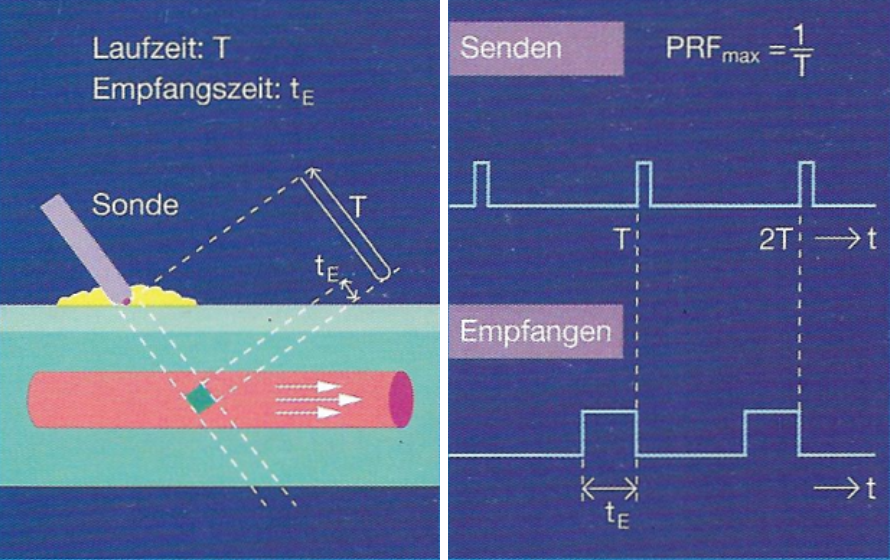
\includegraphics[width=0.7\textwidth]{pwdoppler.png}
         \caption{Zeitliche Zusammenhänge beim Pulsed-Wave-Dopplerverfahren.}\label{fig:pwdoppler}
      \end{figure}

   \subsection{Analyse des Spektrums und Signalverarbeitung}\label{subsec:spektrale-analyse}

      Das von den sich bewegenden Blutzellen zurückgeworfene Echo besteht aus einer hochfrequenten Trägerwelle mit der Sendefrequenz \(f_Q\), die durch verschiedene Doppler-Frequenzanteile \(\Delta f\) moduliert ist. Da der Blutfluss über den Gefäßquerschnitt keine einheitliche Geschwindigkeit besitzt, entstehen mehrere unterschiedliche Dopplerfrequenzen. Dies gilt bereits für laminare Strömungen mit parabolischem Geschwindigkeitsprofil und in noch stärkerem Maß für turbulente Flüsse, bei denen lokal stark unterschiedliche Geschwindigkeiten und sogar Richtungsumkehr auftreten können (vgl. Abbildung~\ref{fig:laminar-turbulent}).
      \\
      Um aus dem Echosignal Flussgeschwindigkeit und -richtung bestimmen zu können, muss zunächst die Dopplerfrequenzverschiebung \(\Delta f\) isoliert werden. Ist \(\Delta f\) bekannt, kann durch Umstellen der Doppler-Gleichung\eqref{eq:doppler-deltaf-standard} die Strömungsgeschwindigkeit berechnet
      werden:
      \begin{equation}
         v \approx \frac{\Delta f\,c}{2 f_Q \cos(\alpha)} .
         \label{eq:geschwindigkeit-aus-doppler}
      \end{equation}

      Zur Bestimmung von \(\Delta f\) wird das aufgezeichnete Echosignal frequenzanalytisch untersucht. Die Doppleranteile werden im Frequenzspektrum sichtbar gemacht, indem die Amplitude (Signalstärke) als Funktion der Frequenz dargestellt wird. Zur Berechnung dieses diskreten Spektrums wird in der Praxis meist die Fast-Fourier-Transformation (FFT) eingesetzt, eine effiziente Implementierung der diskreten Fourier-Transformation (DFT). Die FFT zerlegt das Zeitsignal in seine einzelnen Frequenzanteile; hohe Amplituden in einem Frequenzbereich entsprechen einem großen Blutvolumen, das sich mit der zugehörigen Geschwindigkeit bewegt.

      \begin{figure}[htbp]
         \centering
         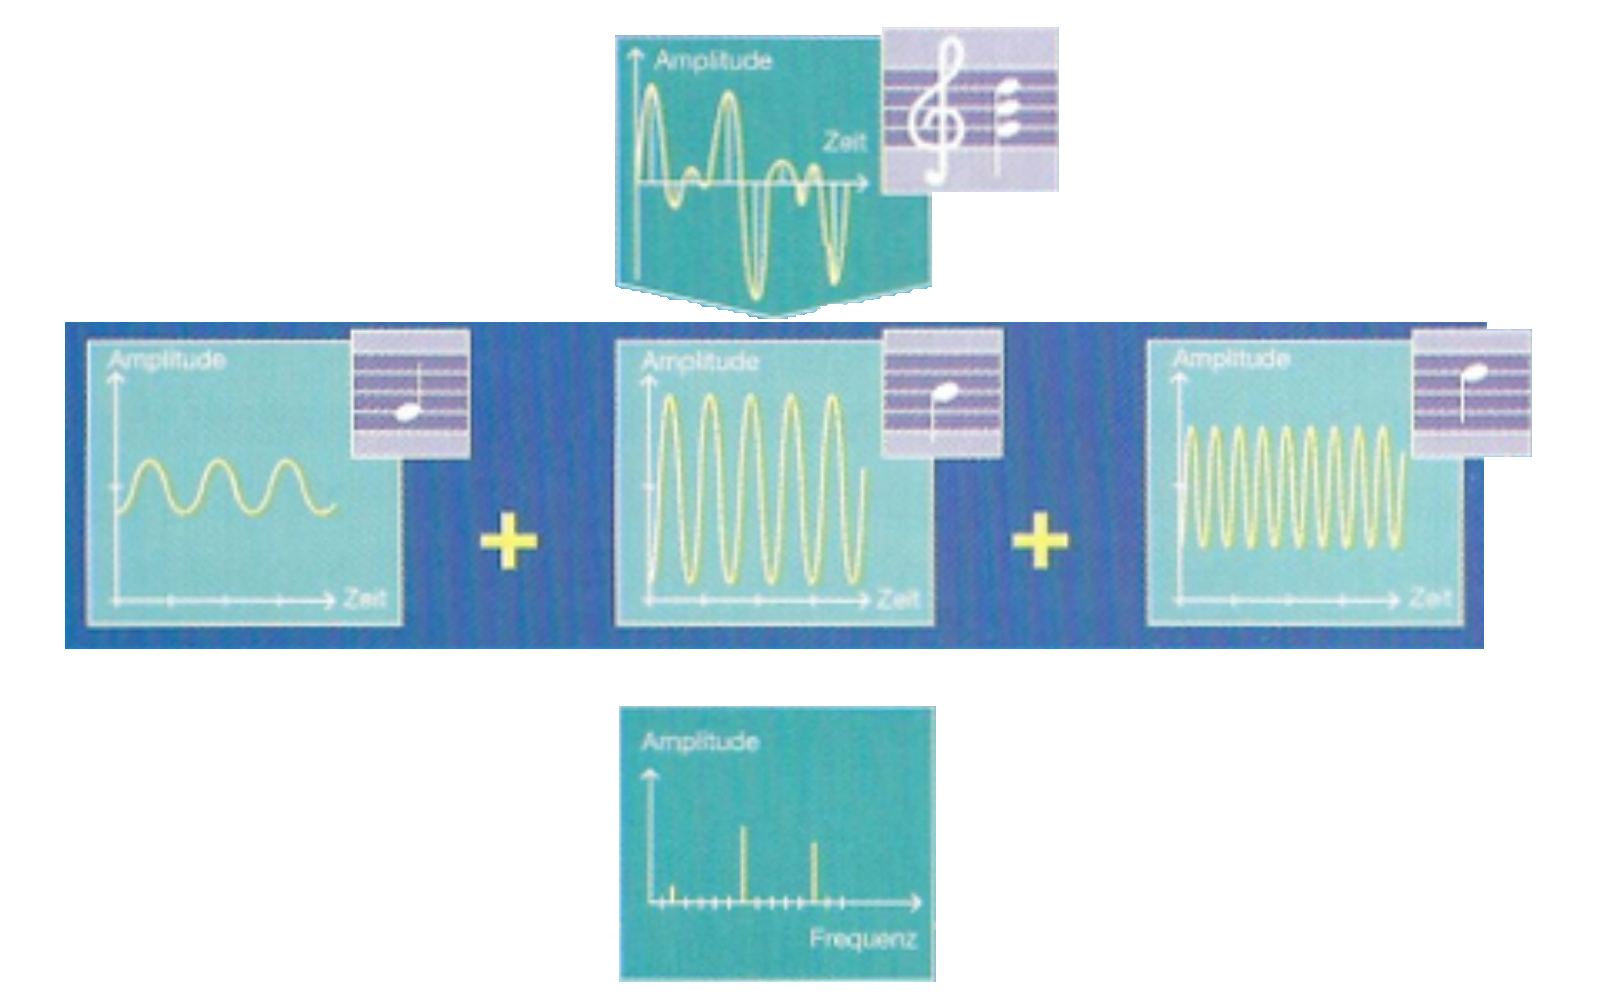
\includegraphics[width=0.7\textwidth]{fft.png}
         \caption{Frequenzanalyse mittels Fast-Fourier-Transformation.}\label{fig:fft-akkord}
         % ich habe das versucht mit tikz zu zeichnen, aber das wurde mir dann doch zu kompliziert...
      \end{figure}

      \begin{figure}[htbp]
         \centering
         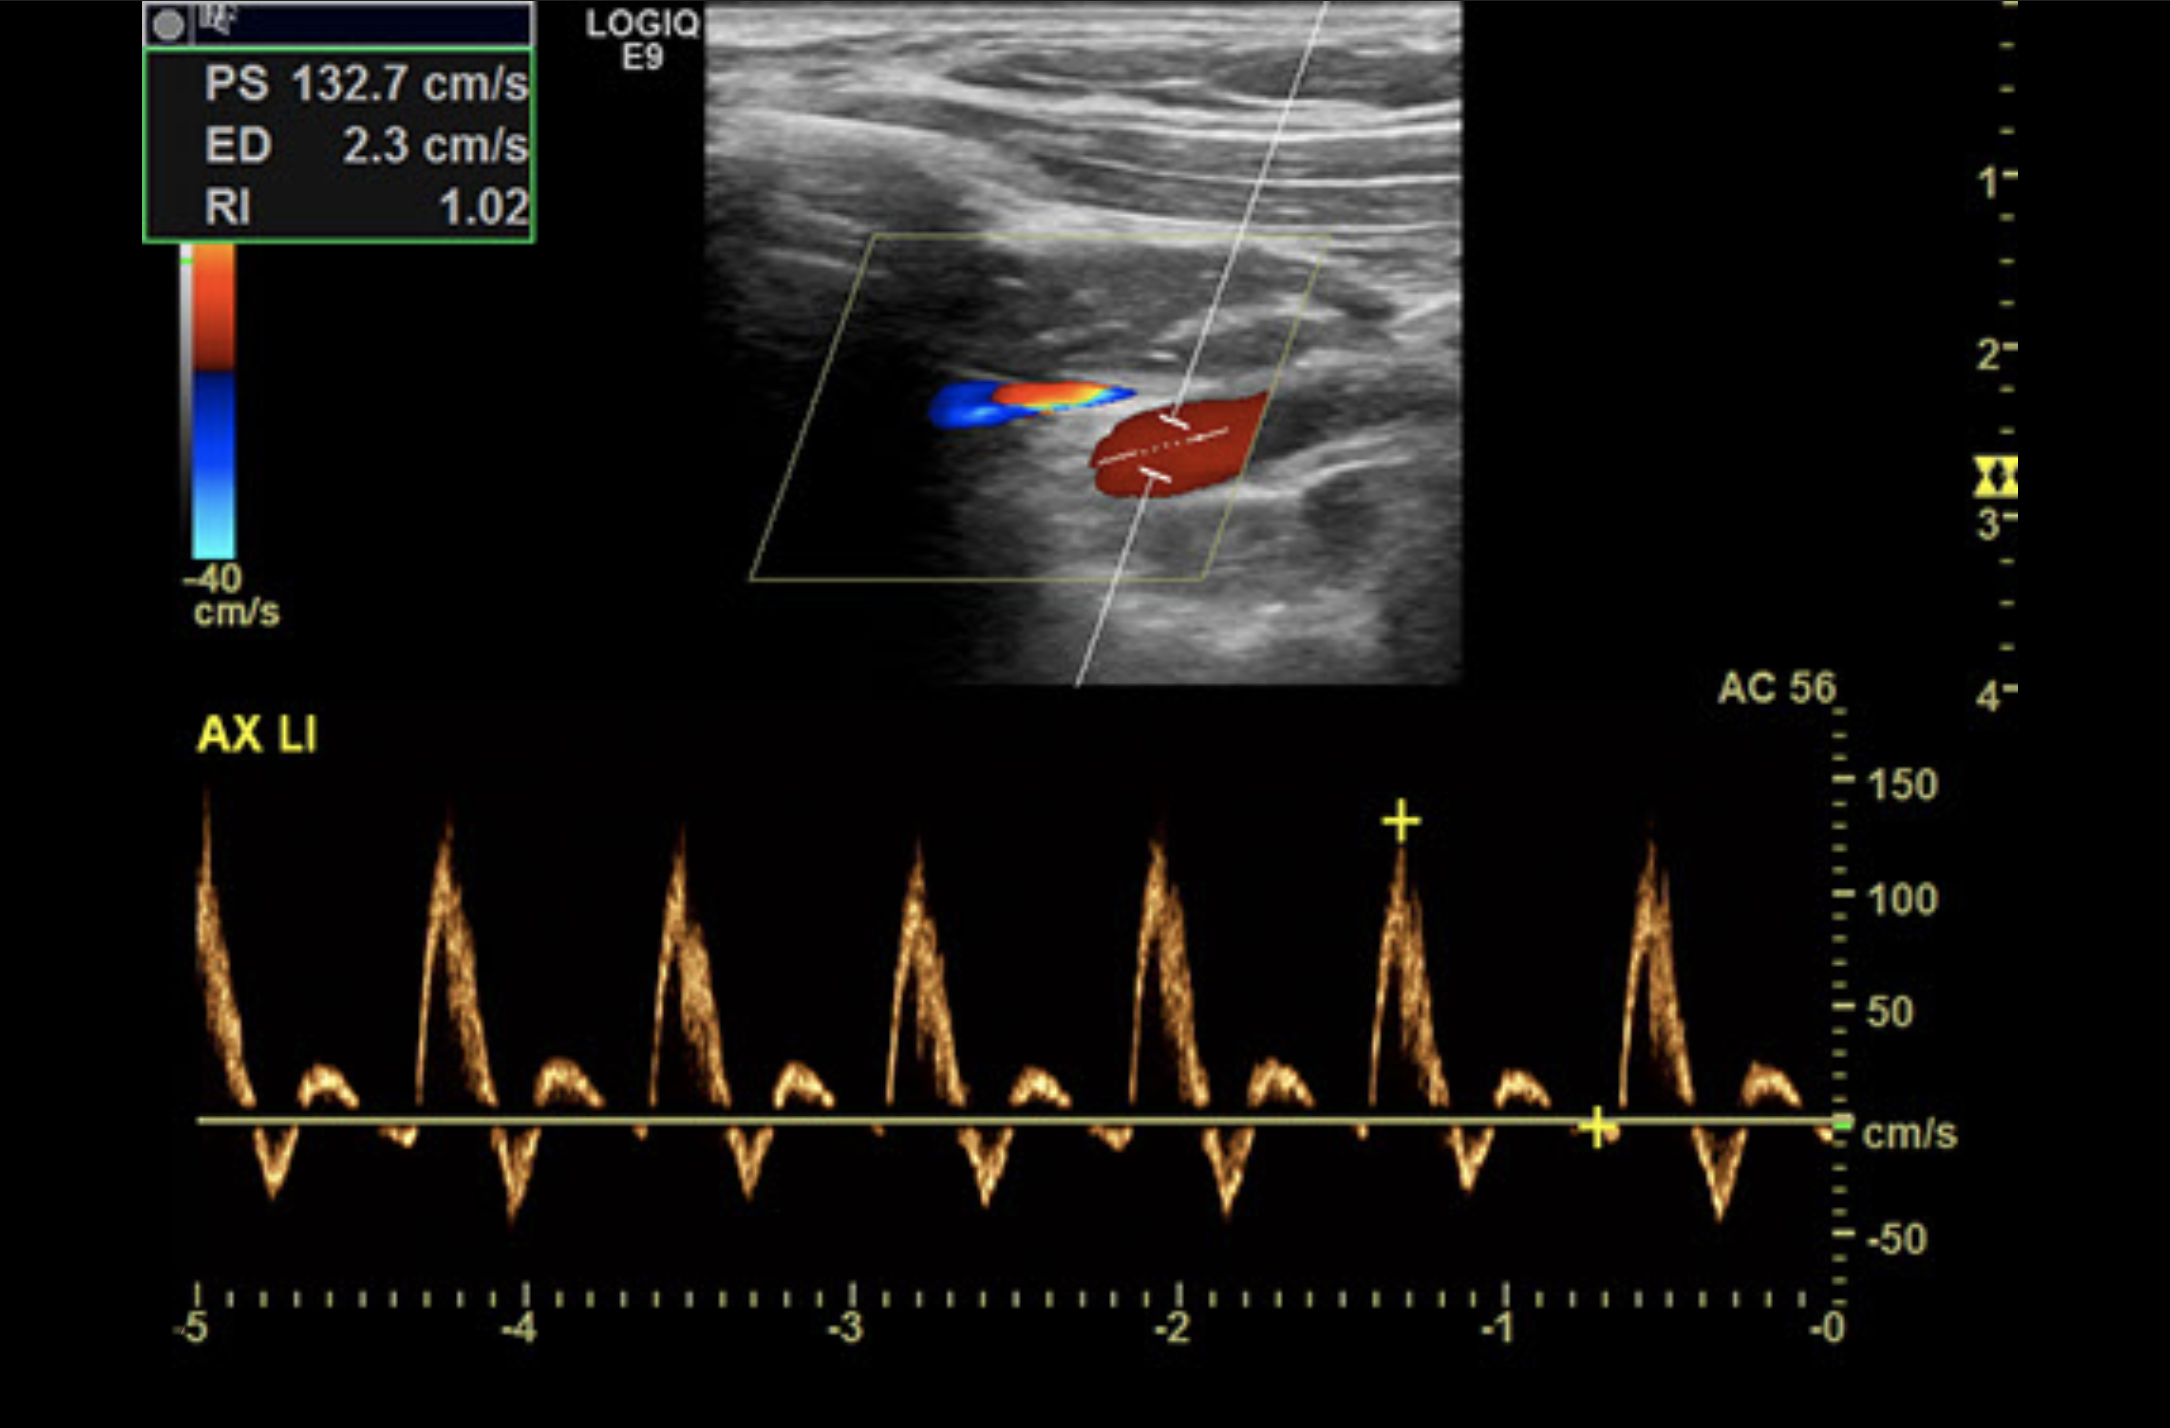
\includegraphics[width=0.7\textwidth]{zeitdoppler.png}
         \caption{Frequenz-Zeit-Spektrum (Spektogramm) einer Arterie}\label{fig:spektrogramm}
         %Quelle Zeitdoppler: https://gefaessmanual.de/?page_id=13008 oder das Bild nehmen https://ultraschallkurs.aerzteverlag.de/auflage-7/buchabbildungen/22-dopplersonografie-peripherer-arterien/i/pic/116/
      \end{figure}

      Die Funktionsweise der FFT lässt sich anschaulich an einem musikalischen Akkord erläutern (vgl. Abbildung~\ref{fig:fft-akkord}). Zu Beginn liegt ein Zeitsignal vor, das aus der Überlagerung von drei verschiedenen Tönen besteht. Jeder Ton besitzt eine eigene Frequenz sowie eine bestimmte Amplitude und trägt damit unterschiedlich stark zum Gesamtklang bei. Durch Anwendung der FFT wird dieses Zeitsignal in seine drei Frequenzanteile aufgespalten, die anschließend mit ihren jeweiligen Amplituden im Spektrum dargestellt werden können. Je höher die Amplitude bei einer Frequenz, desto größer ist der Anteil dieses Tons am Akkord. Genau denselben Mechanismus nutzt man bei der Doppler-Sonographie: Anstelle der Musiktöne treten die unterschiedlichen Geschwindigkeitsanteile des Blutflusses auf. Auf Basis des so gewonnenen Spektrums lassen sich die Hauptfrequenzverschiebungen ablesen und daraus die entsprechenden Blutgeschwindigkeiten bestimmen.
      \\
      Im Frequenz-Zeit-Spektrum (Spektrogramm) kann zusätzlich der zeitliche Verlauf der Spektralanteile dargestellt werden. Die Amplitude der jeweiligen Frequenz wird hierbei in Grau- oder Farbstufen kodiert, sodass hohe Signalanteile als besonders helle bzw.\ intensive Bereiche erscheinen (vgl. Abbildung~\ref{fig:spektrogramm}). Für klinische Anwendungen werden die Frequenzverschiebungen häufig bereits in Geschwindigkeiten umgerechnet, sodass pathologische Beschleunigungen des Blutflusses direkt erkennbar sind.

   \subsection{Messbare Parameter und deren Verwendung}\label{subsec:messbare-parameter}

      Aus dem Doppler-Frequenzspektrum lassen sich mehrere Kenngrößen ableiten, die in der klinischen Praxis zur Beurteilung der Hämodynamik herangezogen werden:
      \begin{itemize}
         \item Systolische Maximalfrequenz als Maß für die maximale
               Strömungsgeschwindigkeit während der Systole und zur Abschätzung des
               Stenosegrades
         \item Enddiastolische Maximalfrequenz zur Beurteilung von Stenosen und des
               diastolischen Strömungsmusters
         \item Gemittelte Strömungsgeschwindigkeit über einen Herzzyklus
         \item Intensitätsgewichtete mittlere Strömungsgeschwindigkeit als Grundlage
               für die Berechnung des Volumenflusses
         \item Varianz bzw.\ spektrale Verbreiterung des Frequenzspektrums als Maß
               für Strömungsstörungen und Turbulenzen.
      \end{itemize}


   \subsection{Dopplerwinkel und Brechungsgesetz}\label{subsec:dopplerwinkel}

      Für die quantitative Blutflussmessung mittels Doppler-Sonographie ist der sogenannte Dopplerwinkel~\(\alpha\) entscheidend, also der Winkel zwischen Strömungsrichtung im Gefäß und Ausbreitungsrichtung der Schallwelle im Blut. Idealisiert wird angenommen, dass die Gefäße parallel zur Hautoberfläche verlaufen und die Haut lokal eben ist. Die Sonde wird mit einem definierten Einschallwinkel~\(\beta\) relativ zur Lotrechten auf die Hautoberfläche aufgesetzt.

      In der Doppler-Gleichung für die Geschwindigkeitsbestimmung (vgl.~Gleichung~\eqref{eq:geschwindigkeit-aus-doppler}) tritt der Faktor \(\cos(\alpha)\) im Nenner auf. Steht der Schallstrahl senkrecht auf dem Gefäß (\(\alpha = 90^\circ\)), gilt \(\cos(90^\circ) = 0\), und es ergibt sich keine messbare Frequenzverschiebung. Je kleiner \(\alpha\) gewählt wird, das heißt je stärker der Schallstrahl in Strömungsrichtung ausgerichtet ist, desto größer wird die beobachtete Frequenzverschiebung~\(\Delta f\) und desto genauer kann die Strömungsgeschwindigkeit~\(v\) bestimmt werden. In der klinischen Praxis werden Dopplerwinkel im Bereich von etwa \(30^\circ\) bis \(60^\circ\) angestrebt, weil sehr flache Winkel geometrisch meist nicht realisierbar sind und sehr steile Winkel zu großen Fehlern in \(v\) führen.
      \\
      Beim Übergang des Schalls von einem Medium in ein anderes (z.\,B.\ von Weichteilgewebe in das mit Blut gefüllte Gefäßlumen) wird der Schallstrahl aufgrund der unterschiedlichen Schallgeschwindigkeiten gebrochen. Für die Winkel zur Lotrechten gilt das Brechungsgesetz
      \begin{equation}
         \frac{c_D}{c_F} = \frac{\sin(\beta)}{\sin(\delta)},
         \label{eq:brechung}
      \end{equation}
      wobei \(\beta\) der Einschallwinkel in Medium~\(D\) (z.\,B.\ Weichteile), \(\delta\) der Brechungswinkel in Medium~\(F\) (Blut) und \(c_D\) bzw.\ \(c_F\) die jeweiligen Schallgeschwindigkeiten sind.
      \\
      Da das Gefäß parallel zur Hautoberfläche verläuft, ergibt sich aus der Geometrie des Strahlverlaufs, dass der Dopplerwinkel~\(\alpha\) zwischen Schallrichtung im Gefäß und Strömungsrichtung
      \begin{equation*}
         \alpha = 90^\circ - \delta
      \end{equation*}
      beträgt. Setzt man nun \(\delta = \arcsin\!\bigl((c_F/c_D)\,\sin\beta\bigr)\), wie es aus Gleichung~\eqref{eq:brechung} folgt, so erhält man
      \begin{equation}
         \alpha = 90^\circ - \arcsin\!\left(\frac{c_F}{c_D}\,\sin(\beta)\right).
         \label{eq:dopplerwinkel}
      \end{equation}
      Der so bestimmte Dopplerwinkel~\(\alpha\) ist in die Doppler-Gleichung einzusetzen und stellt die relevante Größe für die korrekte Berechnung der Blutflussgeschwindigkeit dar.

      \begin{figure}[ht]
         \centering
         \begin{tikzpicture}

         %%%%%%%%%%%%%%%%%%%%%%%%%%%%%%%%%%%%%%%%%%%%%%%%%%%%%%%%%%%%%%%%%%%%%%
         % Parameter
         %%%%%%%%%%%%%%%%%%%%%%%%%%%%%%%%%%%%%%%%%%%%%%%%%%%%%%%%%%%%%%%%%%%%%%
         \def\xmin{-6}
         \def\xmax{6}
         \def\yober{0}
         \def\yunter{-4}
         \def\ytiefe{-2.5}
         \def\greenFrac{0.4}
         \def\blueStartFrac{0.9}
         \def\blueEndFrac{0.5}
         \def\arrowFrac{0.8}

         % gemeinsamer oberer Punkt der vertikalen gestrichelten Linie
         \coordinate (Ytop) at (0,4);

         % Stils für Wellenlinie und Pfeilsegmente
         \tikzset{
            wave/.style={
            decorate,
            decoration={snake, amplitude=3pt, segment length=8pt},
            line width=1.8pt
            },
            arrowseg/.style={
            line width=1.8pt,
            -{Latex[length=3mm]}
            }
         }

         %%%%%%%%%%%%%%%%%%%%%%%%%%%%%%%%%%%%%%%%%%%%%%%%%%%%%%%%%%%%%%%%%%%%%%
         % Hintergrund
         %%%%%%%%%%%%%%%%%%%%%%%%%%%%%%%%%%%%%%%%%%%%%%%%%%%%%%%%%%%%%%%%%%%%%%
         \fill[gray!15] (\xmin,\yunter) rectangle (\xmax,\yober);

         \draw[very thick] (\xmin,\yober) -- (\xmax,\yober);
         \draw[very thick] (\xmin,\yunter) -- (\xmax,\yunter);

         \draw[dashed] (0,\yunter) -- (Ytop);
         \draw[dashed] (\xmin,\ytiefe) -- (\xmax,\ytiefe);

         % 45°-Gerade
         \coordinate (IncStart) at ($(Ytop)+(-4,0)$);
         \coordinate (IncEnd)   at (2.5,\ytiefe);
         \draw[thick] (IncStart) -- (IncEnd);

         \coordinate (Interface) at (0,\yober); % (0,0)

         % %%%%%%%%%%%%%%%%%%%%%%%%%%%%%%%%%%%%%%%%%%%%%%%%%%%%%%%%%%%%%%%%%%%%%%
         % Winkel beta zwischen fallender Gerade und y-Achse (oben)
         % %%%%%%%%%%%%%%%%%%%%%%%%%%%%%%%%%%%%%%%%%%%%%%%%%%%%%%%%%%%%%%%%%%%%%%
         \def\betaradius{1.6}

         % Bogen von 90° (y-Achse nach oben) nach 135° (Richtung fallende Gerade)
         \draw[thick]
         (Interface) ++(90:\betaradius) arc (90:135:\betaradius);

         % Label beta im Bogen
         \node at ($(Interface)+(112.5:1.3)$) {$\beta$};

         % %%%%%%%%%%%%%%%%%%%%%%%%%%%%%%%%%%%%%%%%%%%%%%%%%%%%%%%%%%%%%%%%%%%%%%
         % Winkel delta zwischen y-Achse (nach unten) und grüner Geraden
         % %%%%%%%%%%%%%%%%%%%%%%%%%%%%%%%%%%%%%%%%%%%%%%%%%%%%%%%%%%%%%%%%%%%%%%
         \def\deltaradius{1.6}

         % Bogen von 270° (y-Achse nach unten) nach 315° (Richtung grüne Gerade)
         \draw[thick]
         (Interface) ++(270:\deltaradius) arc (270:315:\deltaradius);

         % Label delta im Bogen
         \node at ($(Interface)+(292.5:1.3)$) {$\delta$};

         % %%%%%%%%%%%%%%%%%%%%%%%%%%%%%%%%%%%%%%%%%%%%%%%%%%%%%%%%%%%%%%%%%%%%%%
         % ROT: Start → Mid (Schlange), Mid → End (gerade + Pfeil)
         % %%%%%%%%%%%%%%%%%%%%%%%%%%%%%%%%%%%%%%%%%%%%%%%%%%%%%%%%%%%%%%%%%%%%%%
         \coordinate (RedStart) at ($(Interface)!0.8!(IncStart)$);
         \coordinate (RedEnd)   at (Interface);
         \coordinate (RedMid)   at ($(RedStart)!\arrowFrac!(RedEnd)$);

         \draw[wave,red] (RedStart) -- (RedMid);
         \draw[arrowseg,red] (RedMid) -- (RedEnd);

         % %%%%%%%%%%%%%%%%%%%%%%%%%%%%%%%%%%%%%%%%%%%%%%%%%%%%%%%%%%%%%%%%%%%%%%
         % GRÜN
         % %%%%%%%%%%%%%%%%%%%%%%%%%%%%%%%%%%%%%%%%%%%%%%%%%%%%%%%%%%%%%%%%%%%%%%
         \coordinate (GreenStart) at (Interface);
         \coordinate (GreenEnd)   at ($(Interface)!\greenFrac!(IncEnd)$);
         \coordinate (GreenMid)   at ($(GreenStart)!\arrowFrac!(GreenEnd)$);

         \draw[wave,green!60!black] (GreenStart) -- (GreenMid);
         \draw[arrowseg,green!60!black] (GreenMid) -- (GreenEnd);

         %%%%%%%%%%%%%%%%%%%%%%%%%%%%%%%%%%%%%%%%%%%%%%%%%%%%%%%%%%%%%%%%%%%%%%
         %%% BLAU (gegenläufig)
         %%%%%%%%%%%%%%%%%%%%%%%%%%%%%%%%%%%%%%%%%%%%%%%%%%%%%%%%%%%%%%%%%%%%%%
         \coordinate (BlueStart) at ($(Interface)!\blueStartFrac!(IncEnd)$);
         \coordinate (BlueEnd)   at ($(Interface)!\blueEndFrac!(IncEnd)$);
         \coordinate (BlueMid)   at ($(BlueStart)!\arrowFrac!(BlueEnd)$);

         \draw[wave,blue] (BlueStart) -- (BlueMid);
         \draw[arrowseg,blue] (BlueMid) -- (BlueEnd);

         %%%%%%%%%%%%%%%%%%%%%%%%%%%%%%%%%%%%%%%%%%%%%%%%%%%%%%%%%%%%%%%%%%%%%%
         %%% Winkel alpha zwischen gestrichelter Linie und blauer Geraden (unten)
         %%%%%%%%%%%%%%%%%%%%%%%%%%%%%%%%%%%%%%%%%%%%%%%%%%%%%%%%%%%%%%%%%%%%%%
         \def\alpharadius{1.4}

         % Bogen von 135° (Richtung blaue Gerade nach oben-links)
         % nach 180° (gestrichelte Linie nach links)
         \draw[thick]
         (IncEnd) ++(135:\alpharadius) arc (135:180:\alpharadius);

         % Label alpha im Bogen
         \node at ($(IncEnd)+(157.5:1.1)$) {$\alpha$};

         %%%%%%%%%%%%%%%%%%%%%%%%%%%%%%%%%%%%%%%%%%%%%%%%%%%%%%%%%%%%%%%%%%%%%%
         %%% BLAUE KUGEL am Schnittpunkt der Geraden mit der gestrichelten Linie
         %%%%%%%%%%%%%%%%%%%%%%%%%%%%%%%%%%%%%%%%%%%%%%%%%%%%%%%%%%%%%%%%%%%%%%
         \fill[blue] (IncEnd) circle (10pt);

         %%%%%%%%%%%%%%%%%%%%%%%%%%%%%%%%%%%%%%%%%%%%%%%%%%%%%%%%%%%%%%%%%%%%%%
         %%% GESCHWINDIGKEITSVEKTOR v NACH RECHTS
         %%%%%%%%%%%%%%%%%%%%%%%%%%%%%%%%%%%%%%%%%%%%%%%%%%%%%%%%%%%%%%%%%%%%%%
         \draw[very thick,blue,-{Latex[length=3mm]}]
         (IncEnd) -- ++(2,0) node[below] {$v$};

         \end{tikzpicture}

         \caption{Schematische Darstellung einer Welle an einer Grenzfläche mit Einfallswinkel $\beta$ zur Normalen, Brechungswinkel $\delta$ im Medium und Winkel $\alpha$ zwischen Messlinie und reflektierter/gestreuter Welle.}\label{fig:dopplerwinkel}
         \end{figure}

%%%%%%%%%%%%%%%%%%%%%%%%%%%%%%%%%%%%%%%%%%%%%%%%%%%%%%%%%%%%%%%%%%%%%%%%%%%%%%%
%%% Habe das einfach mal eingefügt. Wenn du willst, kannst du das gerne
%%% löschen. 
%%% Habe mir gedacht, wäre schön für die Studenten, mal zu sehen, wie 
%%% das in der Praxis aussieht.
%%%%%%%%%%%%%%%%%%%%%%%%%%%%%%%%%%%%%%%%%%%%%%%%%%%%%%%%%%%%%%%%%%%%%%%%%%%%%%%

\clearpage

   \subsection{Klinischer Exkurs: Farb-Doppler-Sonographie*}\label{subsec:farbdoppler}

      Dieser Abschnitt gibt einen kurzen Einblick in die klinische Anwendung der Doppler-Sonographie und zeigt beispielhaft, wie die zuvor beschriebenen physikalischen Prinzipien in der Praxis genutzt werden. 
      \\
      Dieser Exkurs dient der Veranschaulichung und ist nicht Teil des eigentlichen Versuchs.
      \\
      In der Routinediagnostik wird die spektrale Doppleranalyse häufig mit der Farb-Doppler-Sonographie kombiniert. Dabei dient das B-Bild\footnote{Das B-Bild (B-Mode) bezeichnet das konventionelle zweidimensionale Graustufen-Ultraschallbild, das die anatomische Struktur des untersuchten Gebietes (z.B.\ Gefäße, Organe, Wände) darstellt.} des Gefäßes als anatomische Orientierung, während die lokal gemessenen Dopplerfrequenzverschiebungen \(\Delta f\) farbkodiert überlagert werden.
      \\
      Üblicherweise wird das Vorzeichen der Dopplerfrequenz, also die Bewegungsrichtung relativ zur Sonde, durch zwei Farben dargestellt. Eine Farbe (z.B.\ Rot) kennzeichnet Strömung in Richtung der Sonde, die andere (z.B.\ Blau) Strömung von der Sonde weg.\footnote{Die Zuordnung der Farben ist geräteabhängig und kann vom Untersucher invertiert werden. Entscheidend ist das Vorzeichen von \(\Delta f\).} Die Farbsättigung bzw.\ Helligkeit steht dabei im Wesentlichen für die Größe der Geschwindigkeit. Bereiche mit höherer Geschwindigkeit erscheinen intensiver. Zusätzlich können Aliasing-Effekte an charakteristischen Farbumschlägen erkannt werden.
      \\
      Für den Untersucher hat das zwei unmittelbare Vorteile:
      \begin{itemize}
      \item Es wird auf einen Blick sichtbar, wo sich Blutfluss befindet
      \item Die Flussrichtung relativ zur Sonde ist sofort erkennbar
      \end{itemize}

      \begin{figure}[htbp]
         \centering
         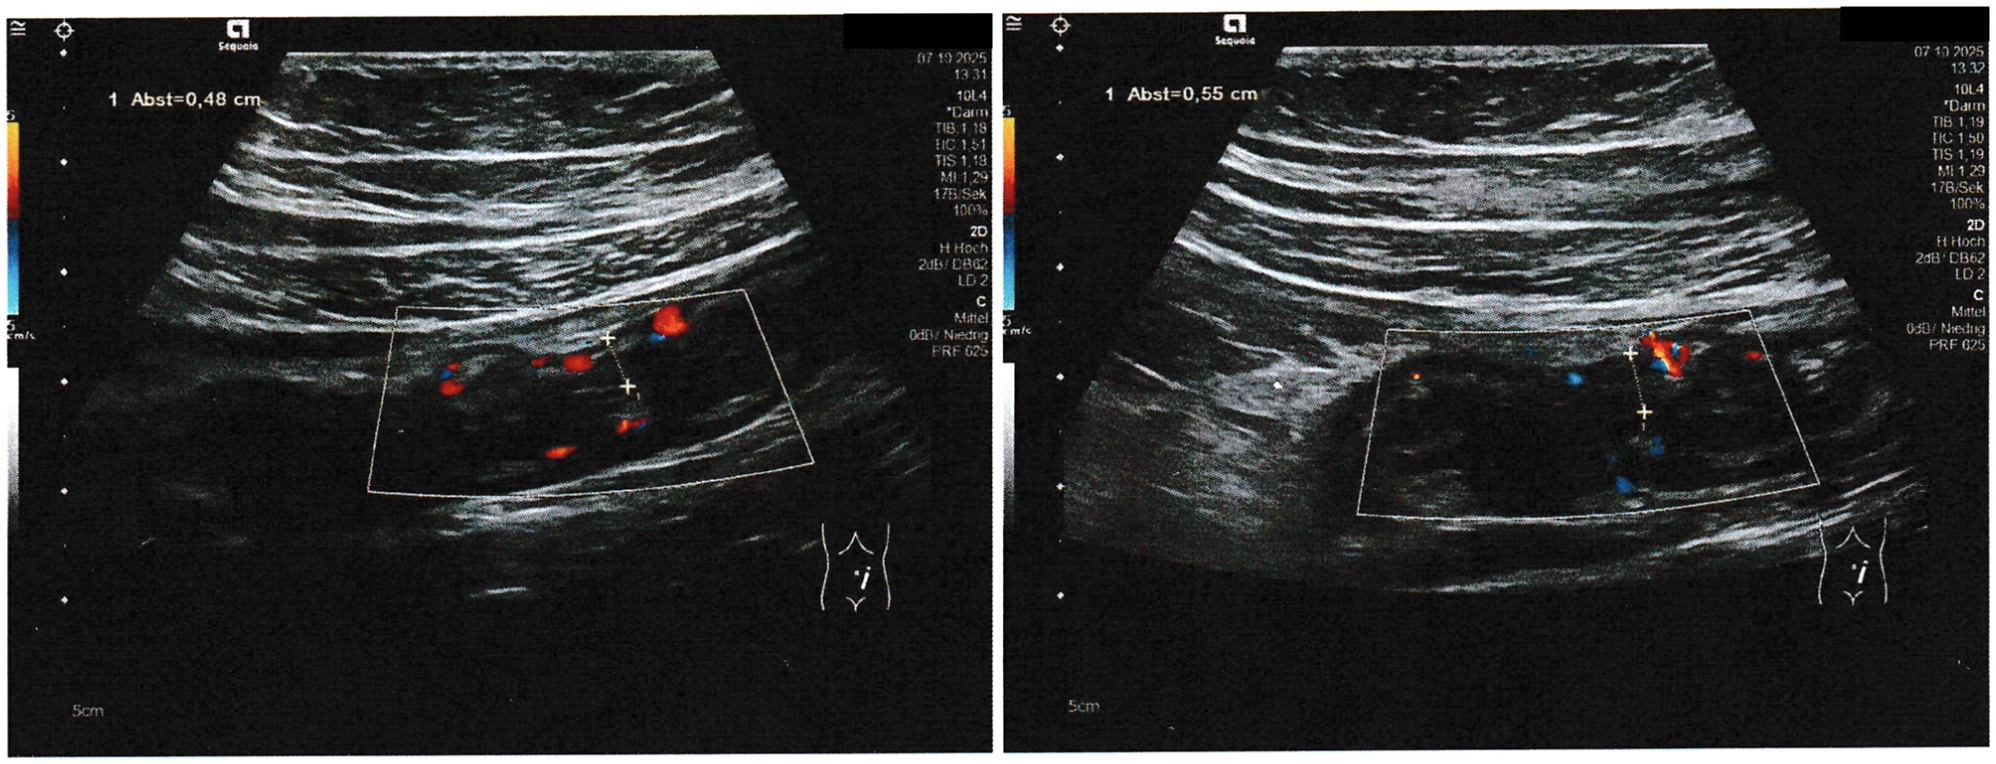
\includegraphics[width=0.7\textwidth]{sono1.png}
         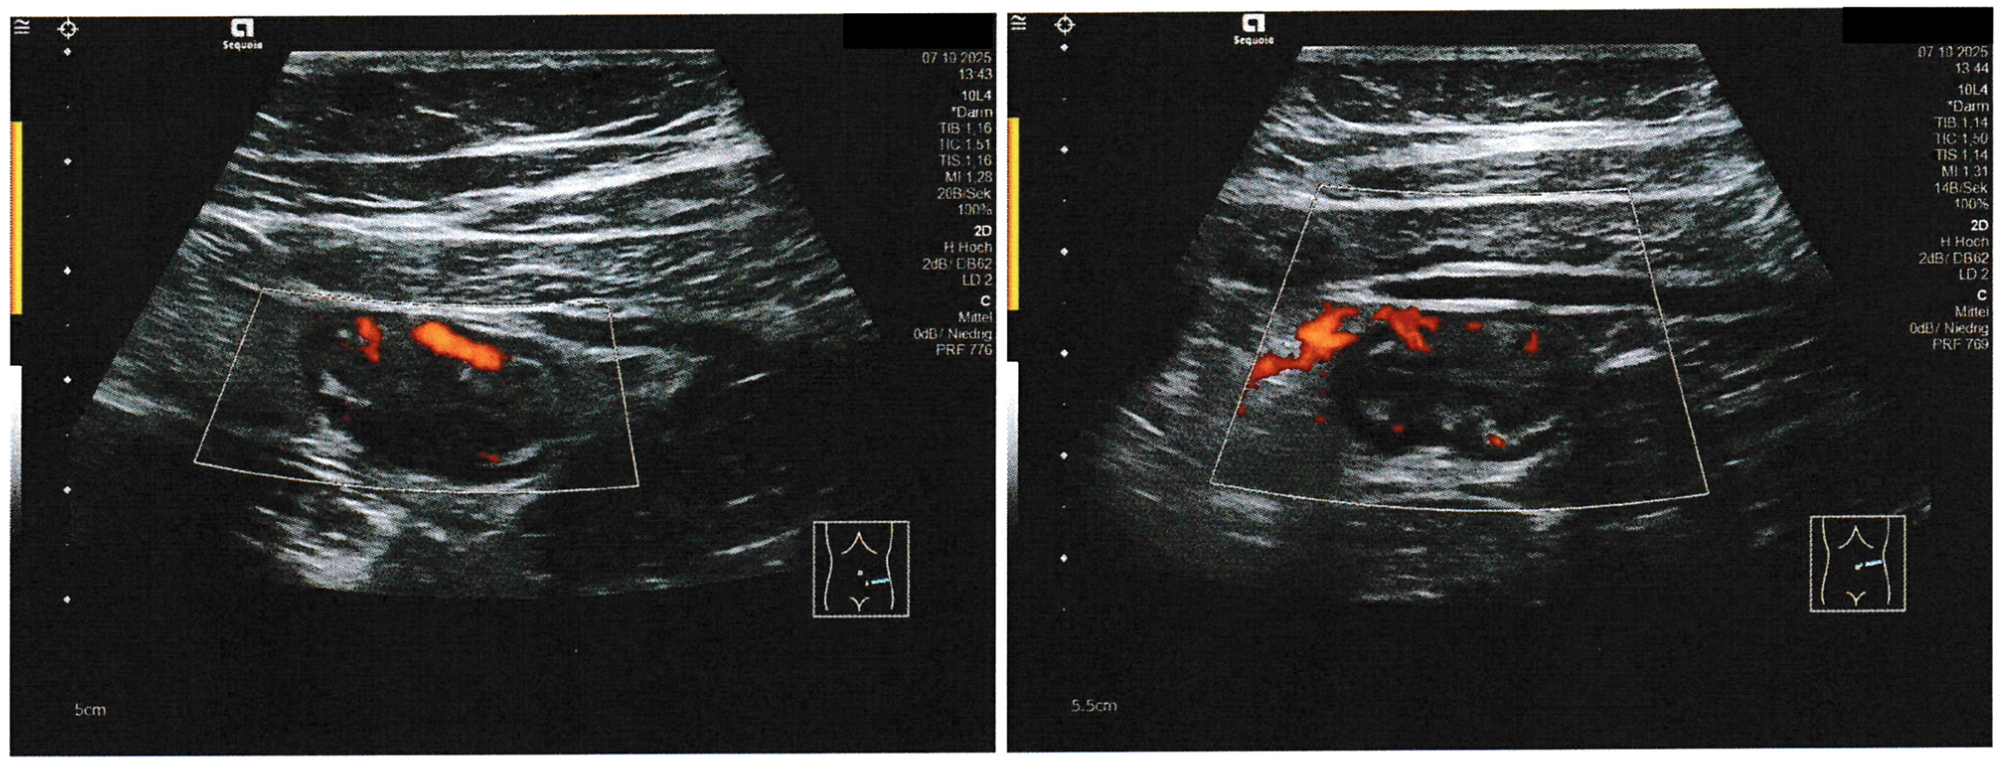
\includegraphics[width=0.7\textwidth]{sono2.png}
         \caption{Farb-Doppler-Sonographie des Colon descendens und Sigmas bei Morbus Crohn mit deutlicher Entzündungsaktivität. Im Vergleich zu einem gesunden Darm ist die Wand verdickt und zeigt eine ausgeprägte Hyperperfusion der Darmwand.}\label{fig:sono}
         % Das sind ********* Bilder aus der Klinik. Habe lediglich oben rechts auf den einzelnen Bildern Namen sowie Geburtsdatum unkenntlich gemacht.
      \end{figure}

%%%%%%%%%%%%%%%%%%%%%%%%%%%%%%%%%%%%%%%%%%%%%%%%%%%%%%%%%%%%%%%%%%%%%%%%%%%%%%%
%%% Nice to know. Kann gerne gelöscht werden, wenn du das nicht möchtest.
%%%%%%%%%%%%%%%%%%%%%%%%%%%%%%%%%%%%%%%%%%%%%%%%%%%%%%%%%%%%%%%%%%%%%%%%%%%%%%%


\end{document}
%% End of file `DEMO-TUDaReport.tex'.
